\chapter{Paralelização dos Mecanismos de E/S do SDDP}
\label{cap:proposta}

Este capítulo apresenta a proposta de paralelização dos mecanismos de
entrada e saída (E/S) do SDDP. A solução substitui o modelo atual,
por uma organização baseada em MPI-IO sobre
o sistema de arquivos Lustre. Nessa abordagem, cada \textit{rank} grava
diretamente seus próprios resultados em regiões independentes do espaço de
saída, evitando a concentração das operações de E/S em um único processo.

O ponto central da proposta é explorar, simultaneamente, o paralelismo da
aplicação MPI e o paralelismo do sistema de arquivos. Como os resultados
produzidos por diferentes \textit{ranks} são independentes, suas escritas
podem ser posicionadas previamente e executadas em paralelo. No Lustre, os
arquivos são distribuídos em \textit{stripes} entre diferentes
\textit{Object Storage Targets} (OSTs); assim, múltiplas escritas
independentes podem ser atendidas por OSTs distintos, aumentando a largura
de banda agregada e reduzindo a contenção observada no modelo com escritor
centralizado.

Dessa forma, a proposta visa reduzir dois gargalos da arquitetura original. O
primeiro é o gargalo de comunicação, pois os dados deixam de ser enviados
ao processo escritor antes de serem persistidos. O segundo é o gargalo de
armazenamento, pois a escrita passa a ser distribuída entre os recursos do
sistema de arquivos paralelo, em vez de ser serializada por um único
\textit{rank}. A Figura~\ref{fig:SDDP_architecture2} sintetiza essa nova
organização.

\section{Uso de MPI-IO com Lustre para escalabilidade de E/S}
Como hipótese para mitigar essas limitações, propõe-se a substituição do modelo atual de E/S por uma abordagem MPI-IO, baseada na interface
MPI-IO em conjunto com o sistema de arquivos distribuído Lustre.

A interface MPI-IO, parte do padrão MPI-2, fornece mecanismos para a
realização de operações de E/S por múltiplos processos MPI sobre arquivos
compartilhados. Diferentemente do modelo tradicional de comunicação ponto a
ponto (\texttt{MPI\_Send}/\texttt{MPI\_Recv}), o MPI-IO permite que cada
processo realize operações diretas de escrita em arquivos, sem a
necessidade de coordenação com um processo único de escrita~\cite{Rwe:99}. Essa flexibilidade
possibilita que os próprios processos responsáveis pela computação escrevam
seus resultados diretamente em disco, utilizando \textit{offsets} distintos
e evitando conflitos de acesso. Isso é particularmente relevante em
aplicações como o SDDP, em que os dados produzidos por cada \textit{rank}
são independentes e podem ser gravados em posições previamente determinadas
de um arquivo compartilhado, ou mesmo em arquivos separados.

Aliado ao MPI-IO, propõe-se o uso do sistema de arquivos Lustre, amplamente
adotado em ambientes de computação de alto desempenho (HPC). O Lustre foi
projetado para oferecer alto rendimento e paralelismo no acesso a arquivos,
distribuindo os dados entre múltiplos servidores de armazenamento (OSTs ---
\textit{Object Storage Targets})~\cite{Pjb:02}. Essa característica torna o
Lustre particularmente eficiente em cenários onde múltiplos nós executam
operações simultâneas de escrita, como se espera com a integração do
MPI-IO. A combinação das duas tecnologias permite que os \textit{ranks}
MPI realizem operações de E/S em paralelo, aproveitando ao máximo a largura
de banda disponível no sistema e reduzindo significativamente os gargalos
causados pela concentração da escrita.

Espera-se que essa nova arquitetura traga ganhos substanciais de
desempenho. Primeiramente, ao eliminar o processo escritor único, a
aplicação poderá distribuir dinamicamente a carga de E/S entre os próprios
processos computacionais, reduzindo a sobrecarga sobre o adaptador de rede
do nó mestre. Em segundo lugar, a redução da dependência de
\textit{buffers} intermediários e de sincronizações entre \textit{ranks}
minimiza a latência entre o término da computação e a persistência dos
resultados. Além disso, a utilização do paralelismo nativo do Lustre deverá
resultar em um melhor aproveitamento dos recursos de armazenamento,
tornando o sistema mais escalável à medida que aumenta o número de nós.
Por fim, essa abordagem alinha-se às boas práticas adotadas em aplicações
científicas de larga escala, promovendo maior portabilidade, eficiência e
adaptabilidade a infraestruturas HPC modernas. A
Figura~\ref{fig:SDDP_architecture2} descreve o funcionamento da proposta.

\section{Organização dos arquivos compartilhados de resultados}
\label{sec:arquivos_compartilhados_sddp}

Os resultados gerados pelo SDDP são organizados em arquivos de saída com
dimensões associadas a estágio, cenário e hora. A dimensão estágio pode
representar meses ou semanas, dependendo da base de dados utilizada, enquanto
as dimensões cenário e hora representam, respectivamente, as realizações
estocásticas simuladas e a discretização horária dos resultados. Assim, cada
registro de saída pode ser identificado por uma tupla
$(e,c,h)$, em que $e$ indica o estágio, $c$ o cenário e $h$ a hora.

Na arquitetura proposta, esses resultados podem ser gravados em arquivos
compartilhados por múltiplos processos MPI. A escrita permanece
independente: cada \textit{rank} calcula previamente a região do arquivo que
corresponde aos resultados sob sua responsabilidade e escreve diretamente
nessa posição por meio de chamadas MPI-IO com \textit{offset} explícito,
como \texttt{MPI\_File\_write\_at} ou sua variante não bloqueante. Com isso,
não é necessário encaminhar todos os blocos para um processo escritor central,
e também não é necessário sincronizar todos os processos em uma operação
coletiva de escrita.

Considerando um arquivo linearizado na ordem estágio--cenário--hora, o
\textit{offset} de um registro pode ser calculado a partir de

\begin{equation}
  \textit{offset}(e,c,h) =
  \textit{base} + (((e \times N_c + c) \times N_h + h) \times S_r),
\end{equation}

em que $N_c$ é o número de cenários, $N_h$ é o número de horas por estágio e
$S_r$ é o tamanho, em bytes, de cada registro de resultado. Essa organização
permite que cada processo escreva em uma região disjunta do arquivo. Quando
um \textit{rank} é responsável por um conjunto contíguo de cenários, horas ou
estágios, a escrita pode ser emitida como um bloco contíguo, evitando o uso de
\textit{strides} ou de \textit{file views} complexas. Essa é uma vantagem
importante para o SDDP, pois reduz a complexidade da descrição do acesso e
favorece requisições maiores ao sistema de arquivos.

A escolha por escrita independente, em vez de escrita coletiva, decorre do
padrão de execução do SDDP. Os subproblemas associados aos cenários podem
terminar em momentos diferentes, e impor uma sincronização global para gravar
resultados pode introduzir espera artificial entre processos. Além disso,
quando os resultados são produzidos em blocos pequenos, sincronizar todos os
\textit{ranks} a cada etapa de escrita pode aumentar a contenção e reduzir a
sobreposição entre computação e E/S. A escrita independente com
\textit{offsets} explícitos preserva a autonomia dos processos e permite que a
aplicação explore uma abordagem assíncrona: os blocos já produzidos podem ser
encaminhados ao sistema de arquivos enquanto outros processos continuam
avançando na computação.

No Lustre, o arquivo compartilhado é dividido em \textit{stripes} distribuídos
entre diferentes OSTs. Portanto, embora a aplicação enxergue um único arquivo
lógico, as regiões escritas por diferentes processos podem ser atendidas por
OSTs distintos, dependendo do \textit{stripe size}, do \textit{stripe count} e
do \textit{offset} de cada escrita. A Figura~\ref{fig:layout_resultados_lustre}
ilustra essa organização: na parte superior, o arquivo lógico é particionado
em regiões de resultados por estágio, cenário e hora; na parte inferior, esses
pedaços são distribuídos em \textit{stripes} sobre os OSTs do Lustre.

\begin{figure}[H]
  \centering
  \resizebox{\textwidth}{!}{%
  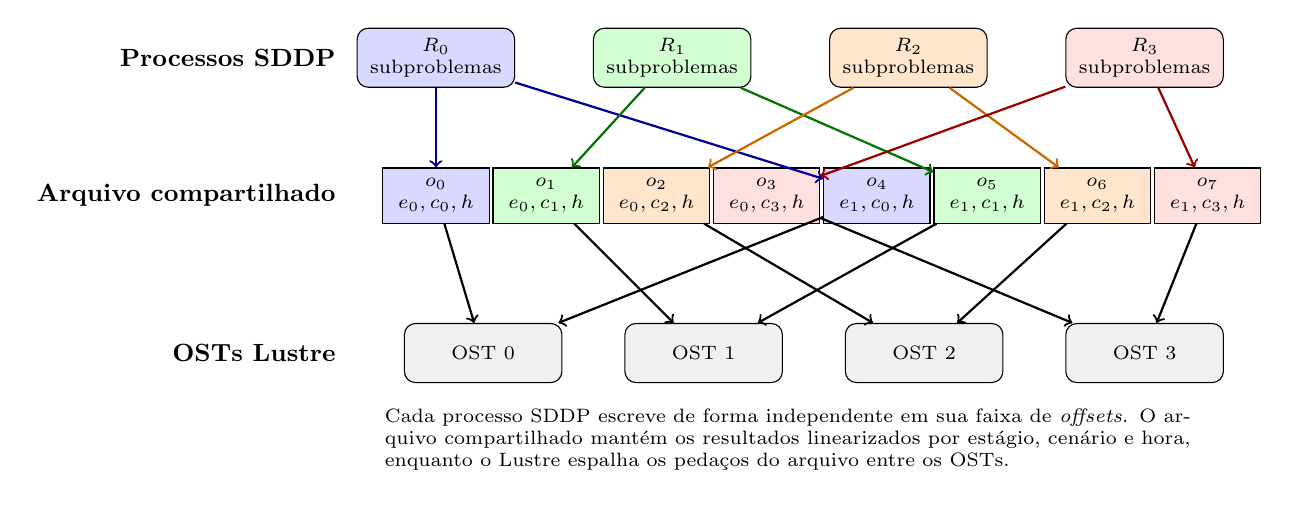
\begin{tikzpicture}[
    font=\scriptsize,
    proc/.style={draw, rounded corners, minimum width=2.0cm, minimum height=0.75cm, align=center},
    seg/.style={draw, minimum width=1.35cm, minimum height=0.7cm, align=center},
    ost/.style={draw, rounded corners, minimum width=2.0cm, minimum height=0.75cm, align=center},
    arr/.style={->, thick}
  ]
    \node[anchor=east, font=\small\bfseries] at (-1.15,2.3) {Processos SDDP};
    \node[proc, fill=blue!15]   (p0) at (0.0,2.3)  {$R_0$\\subproblemas};
    \node[proc, fill=green!18]  (p1) at (3.0,2.3)  {$R_1$\\subproblemas};
    \node[proc, fill=orange!20] (p2) at (6.0,2.3)  {$R_2$\\subproblemas};
    \node[proc, fill=red!12]    (p3) at (9.0,2.3)  {$R_3$\\subproblemas};

    \node[anchor=east, font=\small\bfseries] at (-1.15,0.55)
      {Arquivo compartilhado};
    \node[seg, fill=blue!15]   (f0) at (0.0,0.55) {$o_0$\\$e_0,c_0,h$};
    \node[seg, fill=green!18]  (f1) at (1.4,0.55) {$o_1$\\$e_0,c_1,h$};
    \node[seg, fill=orange!20] (f2) at (2.8,0.55) {$o_2$\\$e_0,c_2,h$};
    \node[seg, fill=red!12]    (f3) at (4.2,0.55) {$o_3$\\$e_0,c_3,h$};
    \node[seg, fill=blue!15]   (f4) at (5.6,0.55) {$o_4$\\$e_1,c_0,h$};
    \node[seg, fill=green!18]  (f5) at (7.0,0.55) {$o_5$\\$e_1,c_1,h$};
    \node[seg, fill=orange!20] (f6) at (8.4,0.55) {$o_6$\\$e_1,c_2,h$};
    \node[seg, fill=red!12]    (f7) at (9.8,0.55) {$o_7$\\$e_1,c_3,h$};

    \draw[arr, blue!60!black]   (p0) -- (f0);
    \draw[arr, blue!60!black]   (p0) -- (f4);
    \draw[arr, green!45!black]  (p1) -- (f1);
    \draw[arr, green!45!black]  (p1) -- (f5);
    \draw[arr, orange!80!black] (p2) -- (f2);
    \draw[arr, orange!80!black] (p2) -- (f6);
    \draw[arr, red!60!black]    (p3) -- (f3);
    \draw[arr, red!60!black]    (p3) -- (f7);

    \node[anchor=east, font=\small\bfseries] at (-1.15,-1.45) {OSTs Lustre};
    \node[ost, fill=gray!12] (ost0) at (0.6,-1.45) {OST 0};
    \node[ost, fill=gray!12] (ost1) at (3.4,-1.45) {OST 1};
    \node[ost, fill=gray!12] (ost2) at (6.2,-1.45) {OST 2};
    \node[ost, fill=gray!12] (ost3) at (9.0,-1.45) {OST 3};

    \draw[arr] (f0) -- (ost0);
    \draw[arr] (f1) -- (ost1);
    \draw[arr] (f2) -- (ost2);
    \draw[arr] (f3) -- (ost3);
    \draw[arr] (f4) -- (ost0);
    \draw[arr] (f5) -- (ost1);
    \draw[arr] (f6) -- (ost2);
    \draw[arr] (f7) -- (ost3);

    \node[align=left, text width=10.5cm] at (4.6,-2.55) {
      Cada processo SDDP escreve de forma independente em sua faixa de
      \textit{offsets}. O arquivo compartilhado mantém os resultados
      linearizados por estágio, cenário e hora, enquanto o Lustre espalha os
      pedaços do arquivo entre os OSTs.
    };
  \end{tikzpicture}
  }
  \caption{Escrita independente dos processos SDDP em um arquivo compartilhado
  e distribuição dos pedaços em OSTs do Lustre.}
  \label{fig:layout_resultados_lustre}
\end{figure}

\begin{figure}[H]
  \centering
  
\includegraphics[width=0.7\textwidth]{SDDP_architecture2.png}
  \caption{Proposta com MPI-IO e Lustre.}
  \label{fig:SDDP_architecture2}
\end{figure}

